% ============================================================
% Capítulo 6: Revisão de Código na Era da IA
% ============================================================
\chapter{Revisão de Código na Era da IA}

\section{Introdução}

Revisão de código é uma das práticas mais poderosas da engenharia de software ---
e uma das mais subestimadas. Muitos times tratam code review como burocracia,
um obstáculo entre o ``git push'' e o deploy. Essa visão está errada.

\begin{itemize}
    \item \textbf{Qualidade}: a revisão é a última linha de defesa antes que um
    bug, uma vulnerabilidade ou uma decisão de design ruim entre em produção.
    \item \textbf{Aprendizado}: cada revisão é uma aula --- o autor aprende com
    o revisor, o revisor aprende com o código do autor.
    \item \textbf{Alinhamento}: revisões garantem que o time está convergindo
    para os mesmos padrões, as mesmas convenções, a mesma direção arquitetural.
    \item \textbf{Propriedade coletiva}: quando todos revisam o código de todos,
    ninguém é dono exclusivo de nenhum módulo. Isso reduz o \textit{bus factor}
    e distribui conhecimento.
\end{itemize}

\subsection{Uma Breve História da Revisão de Código}

A prática de revisar código não nasceu com os Pull Requests do GitHub.

\begin{itemize}
    \item \textbf{1976 --- Inspeções de Fagan}: Michael Fagan, na IBM, formalizou
    o primeiro processo estruturado de revisão de código. Envolviam reuniões
    presenciais, papéis definidos (moderador, autor, inspetor, escriba) e
    métricas rigorosas. Estudos mostraram que encontravam 60--90\% dos defeitos.
    \item \textbf{Anos 1990 --- Revisões por e-mail}: times distribuídos começaram
    a enviar patches por e-mail para revisão. O kernel Linux ainda usa esse modelo.
    \item \textbf{Anos 2000 --- Ferramentas dedicadas}: Gerrit, Crucible, Review
    Board. A revisão ganhou interface gráfica e rastreabilidade.
    \item \textbf{2008+ --- Pull Requests}: GitHub popularizou o modelo de PR,
    democratizando a revisão de código. Hoje é o padrão da indústria.
    \item \textbf{2023+ --- Revisão assistida por IA}: ferramentas como CodeRabbit,
    Amazon CodeGuru, GitHub Copilot e Sourcery oferecem revisão automatizada.
    A IA entra no fluxo, mas não substitui o julgamento humano.
\end{itemize}

\subsection{Por Que a IA Muda o Jogo Mas Não Substitui Humanos}

A IA é extraordinariamente boa em tarefas repetitivas e padronizáveis. Ela
consegue varrer milhares de linhas em segundos procurando padrões conhecidos
de problemas. Mas revisão de código não é apenas encontrar bugs --- é entender
intenção, avaliar design e comunicar conhecimento.

\begin{itemize}
    \item A IA encontra o \textit{o quê}. O humano avalia o \textit{por quê}.
    \item A IA detecta que uma função tem complexidade ciclomática 15. O humano
    decide se isso é aceitável dado o contexto do domínio.
    \item A IA aponta que não há tratamento de erro. O humano decide \textit{qual}
    tratamento de erro faz sentido para aquele caso de uso.
    \item A IA pode gerar mais código do que nunca. Isso significa que precisamos
    de \textit{mais} revisão, não menos.
\end{itemize}

% ============================================================
\section{Princípios de Code Review}

Antes de falar de ferramentas e workflows, precisamos alinhar princípios.
Um processo de revisão sem princípios claros degenera em dois extremos: ou
ninguém revisa de verdade, ou a revisão vira uma arena de egos.

\subsection{Objetivo: Qualidade e Aprendizado, Não Gatekeeping}

\begin{itemize}
    \item A revisão existe para melhorar o código \textbf{e} o time.
    \item Não é um tribunal onde o revisor julga o autor.
    \item Não é um ritual de poder onde o sênior bloqueia o júnior.
    \item Um bom review produz código melhor \textbf{e} pessoas melhores.
    \item Se o autor não aprendeu nada com a revisão, ela foi ineficaz.
    \item Se o revisor não aprendeu nada, ele não prestou atenção.
\end{itemize}

\subsection{Foco em Design, Não em Estilo}

\begin{itemize}
    \item \textbf{Linters e formatadores existem para isso}: ESLint, Prettier,
    Black, Rubocop, gofmt. Se o estilo pode ser automatizado, automatize.
    \item \textbf{Não gaste energia humana em tabulação}: se o time discute se
    usa 2 ou 4 espaços no code review, o processo está desperdiçando capital
    intelectual.
    \item \textbf{Foque no que importa}: o design está correto? A abstração
    faz sentido? Os nomes comunicam intenção? A complexidade é justificada?
    \item \textbf{Regra prática}: se um linter pode pegar, não é assunto de
    code review.
\end{itemize}

\subsection{Feedback Construtivo e Respeitoso}

\begin{itemize}
    \item \textbf{Critique o código, não a pessoa}: ``essa função está fazendo
    coisas demais'' em vez de ``você não sabe dividir responsabilidades''.
    \item \textbf{Sugira, não ordene}: ``que tal extrair essa lógica para um
    serviço?'' em vez de ``refatore isso''.
    \item \textbf{Explique o porquê}: ``esse acoplamento vai dificultar testes
    unitários porque...'' em vez de apenas ``muito acoplado''.
    \item \textbf{Reconheça o bom}: não comente só problemas. ``Gostei dessa
    abstração, ficou bem clara'' motiva e reforça boas práticas.
    \item \textbf{Use perguntas}: ``qual foi o raciocínio para usar herança
    aqui em vez de composição?'' abre diálogo em vez de impor opinião.
\end{itemize}

\subsection{Tamanho Ideal de Pull Request}

O tamanho do PR é um dos fatores mais determinantes para a qualidade da revisão.
PRs grandes demais não recebem revisão real --- recebem um ``LGTM'' cansado.

\begin{table}[htbp]
\centering
\caption{Tamanho Ideal de Pull Request}
\begin{tabular}{lll}
\toprule
\textbf{Linhas Alteradas} & \textbf{Classificação} & \textbf{Qualidade da Revisão} \\
\midrule
1--50    & Pequeno   & Excelente --- revisão rápida e precisa \\
50--200  & Ideal     & Muito boa --- revisor consegue manter contexto \\
200--400 & Aceitável & Boa, mas exige atenção prolongada \\
400--800 & Grande    & Superficial --- revisor perde foco \\
800+     & Enorme    & Ilusória --- ninguém revisa 800 linhas de verdade \\
\bottomrule
\end{tabular}
\end{table}

\begin{itemize}
    \item \textbf{Pesquisa da SmartBear}: revisões de mais de 400 linhas apresentam
    queda drástica na taxa de detecção de defeitos.
    \item \textbf{Regra dos 60 minutos}: após 60 minutos de revisão contínua, a
    eficácia cai significativamente. PRs devem ser revisáveis em menos tempo.
    \item \textbf{Estratégia}: se a feature é grande, divida em PRs incrementais.
    Cada um deve ser funcional e testável independentemente.
\end{itemize}

\subsection{A Mentalidade do Revisor}

\begin{itemize}
    \item Aborde o código com curiosidade, não com desconfiança.
    \item Assuma que o autor tinha boas razões para suas decisões.
    \item Pergunte antes de assumir que algo está errado.
    \item Priorize: nem todo comentário precisa bloquear o merge.
    \item Diferencie entre ``precisa mudar'' e ``eu faria diferente''.
    \item Prefira o prefixo \texttt{nit:} para sugestões opcionais e cosméticas.
\end{itemize}

\subsection{A Mentalidade do Autor}

\begin{itemize}
    \item Não leve feedback para o lado pessoal --- o alvo é o código.
    \item Facilite a vida do revisor: descrição clara, PR pequeno, testes.
    \item Responda todos os comentários, mesmo que seja ``concordo, corrigido''.
    \item Se discorda, argumente com contexto técnico, não com ego.
    \item Agradeça sugestões boas --- reforça a cultura de colaboração.
\end{itemize}

% ============================================================
\section{O Que a IA Revisa Bem}

A IA é particularmente eficaz em categorias de problemas que são detectáveis
por padrões, regras e heurísticas. Essas são tarefas onde a velocidade e
a consistência da IA superam a capacidade humana.

\begin{itemize}
    \item \textbf{Erros de sintaxe e typos}: variáveis com nomes errados,
    parênteses desbalanceados, imports não utilizados. A IA é incansável para
    esses detalhes.

    \item \textbf{Vulnerabilidades de segurança conhecidas}: padrões OWASP como
    SQL injection, XSS, path traversal, uso de funções criptográficas obsoletas.
    A IA foi treinada em milhões de exemplos desses padrões.

    \item \textbf{Violações de convenções}: naming conventions, organização de
    imports, padrões de estrutura de arquivos. Regras codificáveis que humanos
    esquecem.

    \item \textbf{Code smells comuns}: funções longas demais, classes com
    responsabilidades múltiplas, God objects, feature envy, código duplicado.
    A IA detecta padrões estruturais com facilidade.

    \item \textbf{Complexidade ciclomática}: a IA calcula e alerta quando a
    complexidade ultrapassa limiares aceitáveis. McCabe definiu que acima de 10
    merece atenção; acima de 20, refatoração obrigatória.

    \item \textbf{Código morto}: variáveis declaradas mas nunca usadas, funções
    definidas mas nunca chamadas, branches de código inacessíveis.

    \item \textbf{Anti-padrões de performance}: consultas N+1, loops com
    alocação desnecessária, concatenação de strings em loops, falta de paginação,
    operações síncronas que deveriam ser assíncronas.
\end{itemize}

\begin{lstlisting}[language={}, caption={Exemplo de Saída de Revisão por IA}]
## Revisao Automatica - CodeRabbit

### Seguranca [CRITICO]
- Linha 47: SQL injection detectado. Uso de string
  interpolation em query SQL.
  Sugestao: usar prepared statements.

### Performance [AVISO]
- Linha 112-130: Consulta N+1 detectada. Loop faz
  query individual para cada usuario.
  Sugestao: usar batch query ou JOIN.

### Code Smell [INFO]
- Linha 85: Funcao `processarPedido()` tem complexidade
  ciclomatica 18. Considere extrair sub-funcoes.

### Convencoes [INFO]
- Linha 23: Variavel `Dt` nao segue camelCase.
  Sugestao: renomear para `dataTransacao`.
\end{lstlisting}

% ============================================================
\section{O Que Só Humanos Revisam Bem}

Enquanto a IA brilha em padrões, os humanos são insubstituíveis em julgamento.
Essas são as dimensões que exigem contexto, experiência e raciocínio abstrato.

\begin{itemize}
    \item \textbf{Adequação ao domínio de negócio}: o código resolve o problema
    certo? A IA não sabe que ``cliente premium'' no seu sistema tem regras
    específicas de desconto que não estão no código, mas em conversas com o
    product owner.

    \item \textbf{Clareza de intenção}: o código comunica \textit{por que}
    existe, não apenas \textit{o que} faz? Nomes de variáveis, funções e
    classes revelam a intenção do domínio?

    \item \textbf{Decisões de design e arquitetura}: esse serviço deveria ser
    síncrono ou assíncrono? Essa responsabilidade pertence a esta camada?
    Estamos criando acoplamento desnecessário entre módulos?

    \item \textbf{Trade-offs e decisões técnicas}: usamos cache e aceitamos
    eventual inconsistência? Duplicamos dados para melhorar performance de
    leitura? Essas decisões exigem entendimento do contexto e das prioridades.

    \item \textbf{Contexto organizacional}: esse PR afeta o time de data
    science que consome essa API? O time de mobile está esperando esse contrato?
    Há migração de dados planejada que depende disso?

    \item \textbf{Crescimento e conhecimento da equipe}: o júnior que escreveu
    esse código está pronto para aprender sobre esse padrão? A revisão é uma
    oportunidade de mentoria?
\end{itemize}

\begin{table}[htbp]
\centering
\caption{O Que Revisar: IA vs Humano}
\begin{tabular}{p{5.5cm}cc}
\toprule
\textbf{Aspecto da Revisão} & \textbf{IA} & \textbf{Humano} \\
\midrule
Erros de sintaxe e typos            & Excelente & Desnecessário \\
Vulnerabilidades conhecidas (OWASP) & Excelente & Complementar \\
Violações de convenções             & Excelente & Desnecessário \\
Code smells e complexidade          & Muito Bom & Complementar \\
Código morto e imports não usados   & Excelente & Desnecessário \\
Anti-padrões de performance         & Bom       & Essencial    \\
Adequação ao domínio de negócio     & Fraco     & Essencial    \\
Clareza de intenção e naming        & Razoável  & Essencial    \\
Decisões de design e arquitetura    & Fraco     & Essencial    \\
Trade-offs técnicos                 & Fraco     & Essencial    \\
Contexto organizacional             & Inexistente & Essencial  \\
Mentoria e crescimento da equipe    & Inexistente & Essencial  \\
\bottomrule
\end{tabular}
\end{table}

\begin{lstlisting}[language={}, caption={Exemplo de Revisão Humana vs IA}]
## O que a IA comentou:
"Funcao `calcularDesconto()` tem complexidade
 ciclomatica 12. Considere refatorar."

## O que o humano comentou:
"Essa logica de desconto esta duplicada com o
 servico de cupons. Quando o time de marketing
 mudar as regras (e vai mudar no Q2), vamos ter
 que atualizar em dois lugares. Sugiro extrair
 para um DescontoService unico que ambos os
 fluxos consumam. Posso te ajudar com o design
 se quiser."

## Diferenca:
- A IA viu a COMPLEXIDADE (metrica).
- O humano viu o RISCO DE NEGOCIO (contexto).
\end{lstlisting}

% ============================================================
\section{Workflow de Revisão Híbrido}

O workflow mais eficaz combina automação e julgamento humano em etapas
complementares. A IA não substitui o humano --- ela \textit{libera} o humano
para focar no que importa.

\begin{figure}[htbp]
    \centering
    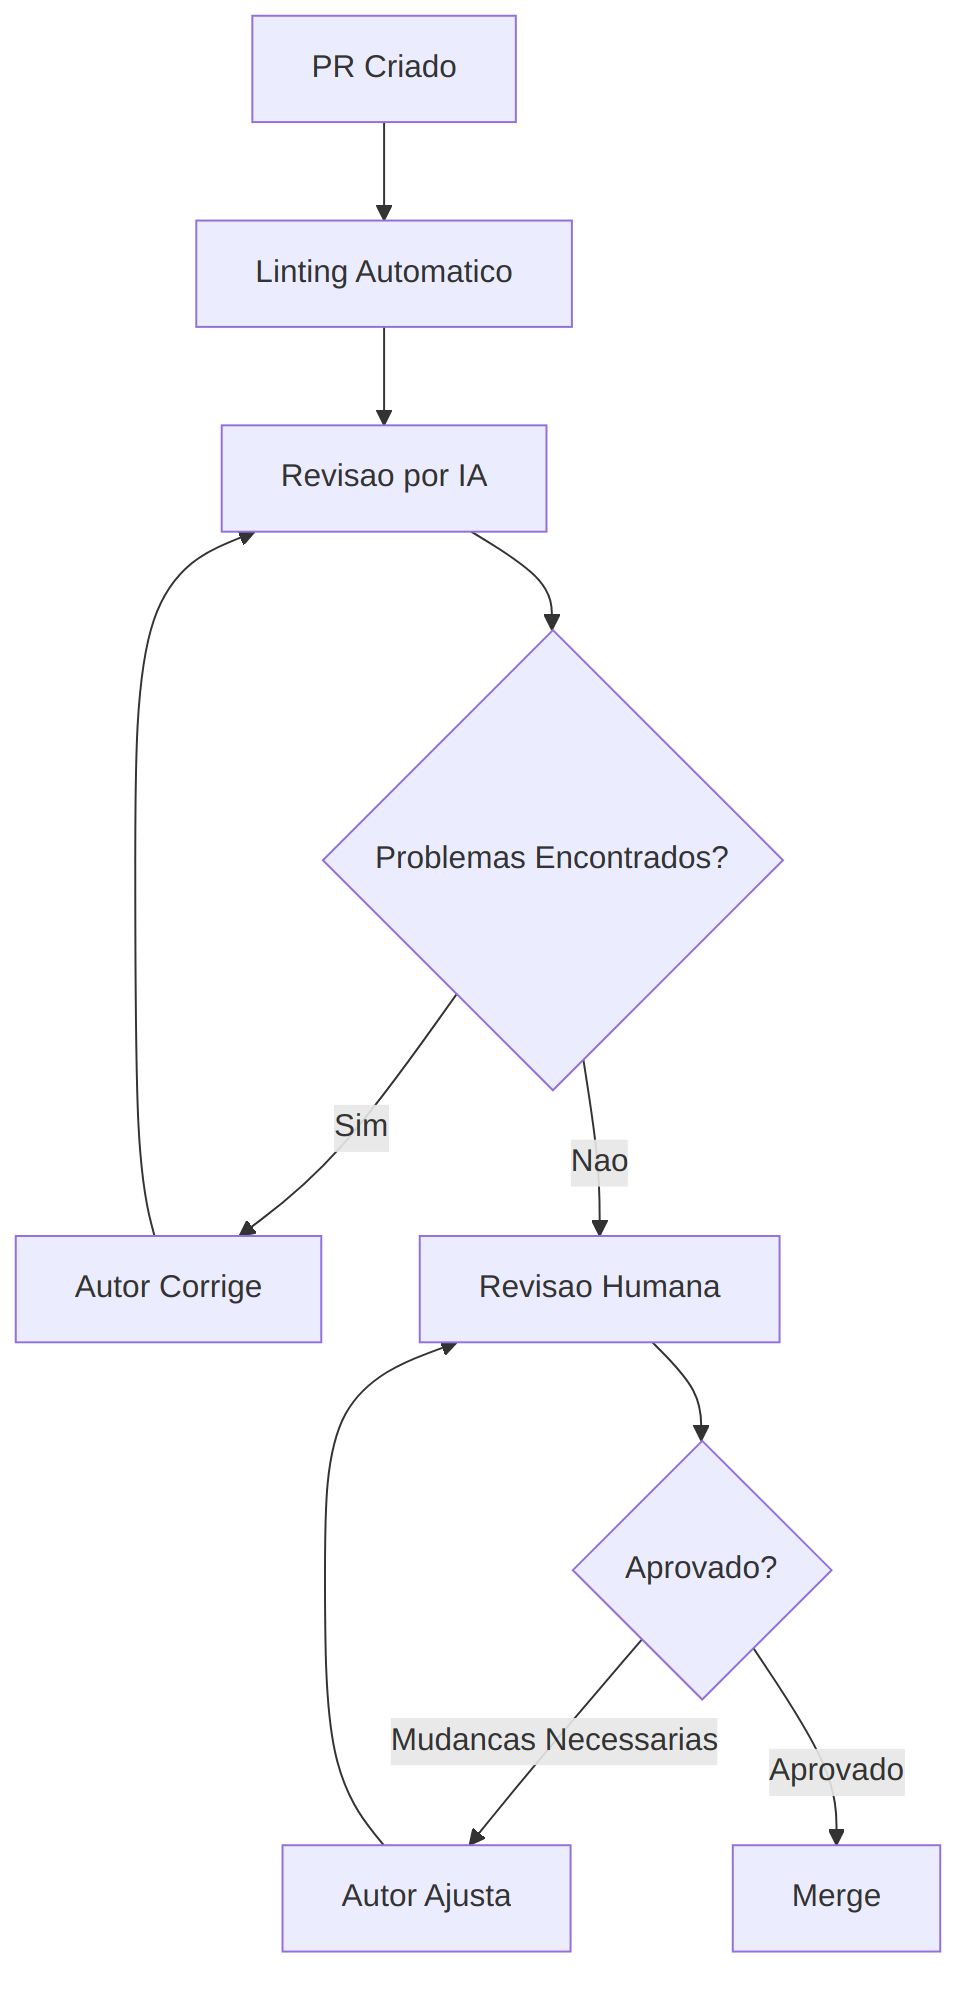
\includegraphics[width=0.85\textwidth]{imagens/06-revisao-codigo-era-ia-01-workflow-de-revisao-hibrido.png}
    \caption{Workflow de Revisão Híbrido}
\end{figure}

\subsection{Passo 1: Linting e Formatação Automáticos}

\begin{itemize}
    \item Executados automaticamente no CI/CD ao criar o PR.
    \item Ferramentas: ESLint, Prettier, Black, Rubocop, gofmt, clang-format.
    \item \textbf{Zero intervenção humana}: se o código não passa no linter,
    o PR não avança. Ponto final.
    \item Idealmente, o desenvolvedor roda essas ferramentas localmente antes
    do push (pre-commit hooks).
\end{itemize}

\subsection{Passo 2: Revisão por IA (Segurança, Bugs, Padrões)}

\begin{itemize}
    \item A IA analisa o diff e produz comentários automatizados.
    \item Foco: segurança, bugs óbvios, code smells, complexidade.
    \item Ferramentas: CodeRabbit, Amazon CodeGuru, SonarQube, Semgrep,
    GitHub Copilot code review, Sourcery.
    \item Os comentários aparecem diretamente no PR, como se fossem de um
    revisor humano.
    \item \textbf{Importante}: configure a sensibilidade. Muitos falsos
    positivos fazem o time ignorar a ferramenta.
\end{itemize}

\subsection{Passo 3: Autor Endereça Achados da IA}

\begin{itemize}
    \item O autor resolve os problemas apontados pela IA antes de solicitar
    revisão humana.
    \item Isso respeita o tempo do revisor humano --- ele não deveria gastar
    energia em problemas que uma máquina já detectou.
    \item Se o autor discorda de um achado da IA, deve justificar com um
    comentário no PR.
\end{itemize}

\subsection{Passo 4: Revisão Humana (Design, Arquitetura, Intenção)}

\begin{itemize}
    \item O revisor humano já recebe o código limpo de problemas triviais.
    \item Foco: design, arquitetura, adequação ao domínio, clareza,
    manutenibilidade, impacto sistêmico.
    \item O revisor lê a descrição do PR, entende o contexto e avalia se a
    solução é adequada --- não apenas se o código ``funciona''.
    \item Idealmente, dois revisores: um do mesmo time (contexto) e um de
    fora (perspectiva fresca).
\end{itemize}

\subsection{Passo 5: Discussão e Aprovação}

\begin{itemize}
    \item Autor e revisores discutem os pontos levantados.
    \item Comentários são resolvidos explicitamente.
    \item Após aprovação, o merge é feito --- preferencialmente com squash
    para manter o histórico limpo.
    \item \textbf{Regra de ouro}: nunca faça merge do próprio PR sem revisão,
    exceto em emergências documentadas.
\end{itemize}

\subsection{Ferramentas do Ecossistema}

\begin{itemize}
    \item \textbf{GitHub Actions}: orquestra o pipeline de CI/CD que inclui
    linting, testes e triggers para revisão por IA.
    \item \textbf{SonarQube}: análise estática profunda, cobertura de código,
    dívida técnica, vulnerabilidades.
    \item \textbf{CodeRabbit}: revisão por IA que comenta diretamente no PR
    com sugestões contextualizadas.
    \item \textbf{Semgrep}: análise estática baseada em regras customizáveis.
    Permite criar regras específicas para seu projeto.
    \item \textbf{Danger}: automação de revisão que verifica metadados do PR
    (tamanho, descrição, labels, changelog).
    \item \textbf{CODEOWNERS}: arquivo do GitHub que define automaticamente
    quem revisa cada parte do código.
\end{itemize}

\begin{figure}[htbp]
    \centering
    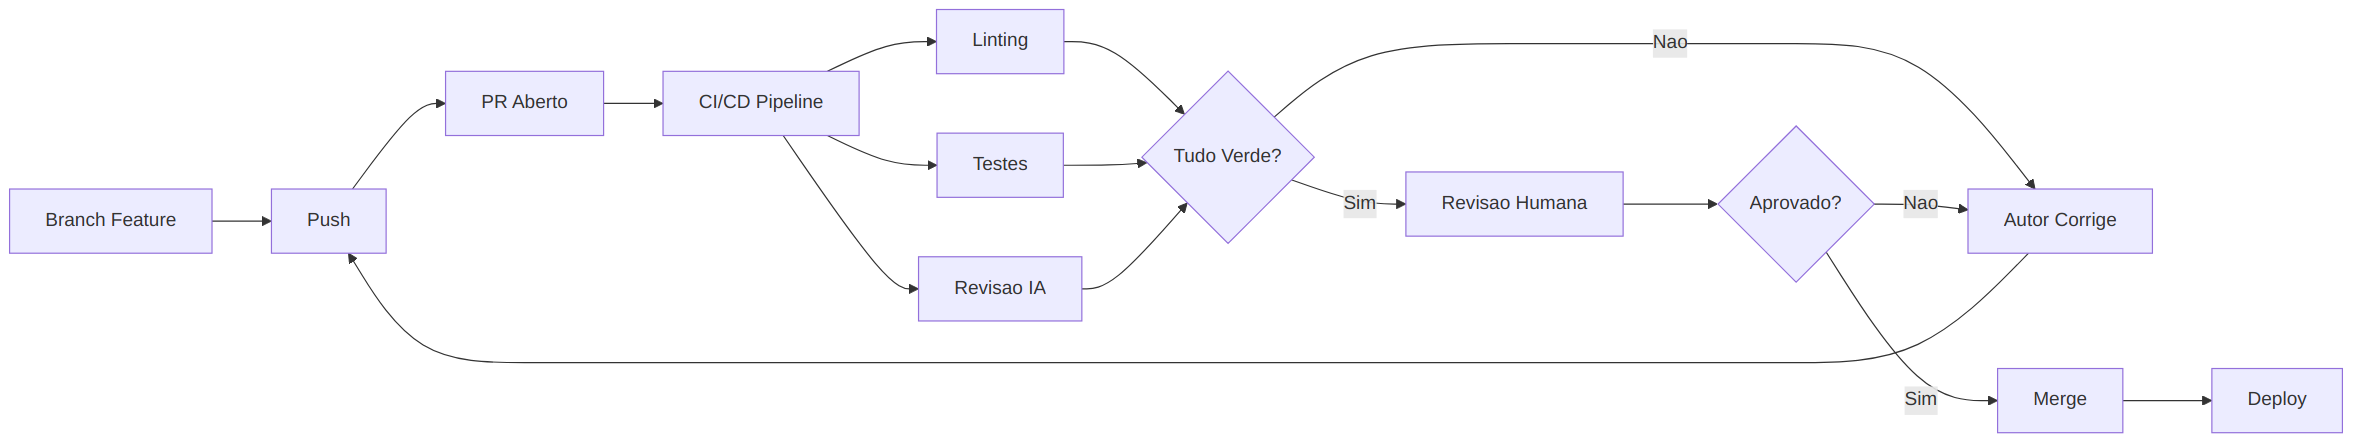
\includegraphics[width=0.85\textwidth]{imagens/06-revisao-codigo-era-ia-02-ciclo-de-vida-de-um-pull-request.png}
    \caption{Ciclo de Vida de um Pull Request}
\end{figure}

% ============================================================
\section{Checklist de Revisão}

Um checklist não substitui o pensamento crítico, mas garante que aspectos
fundamentais não sejam esquecidos. O checklist abaixo combina verificações
automatizáveis (delegáveis à IA) e verificações que exigem julgamento humano.

\begin{table}[htbp]
\centering
\caption{Checklist de Revisão Completo}
\begin{tabular}{p{6cm}p{2.5cm}p{3.5cm}}
\toprule
\textbf{Item de Verificação} & \textbf{Responsável} & \textbf{Categoria} \\
\midrule
O código compila sem erros?                    & IA / CI    & Funcional \\
Os testes existentes continuam passando?       & IA / CI    & Funcional \\
Novos testes foram adicionados?                & Humano     & Testes \\
Os testes cobrem os edge cases?                & Humano     & Testes \\
O código resolve o problema proposto?          & Humano     & Funcional \\
O design é claro e extensível?                 & Humano     & Design \\
Os nomes comunicam intenção?                   & Humano     & Design \\
Há acoplamento desnecessário?                  & Humano     & Design \\
A complexidade é justificada?                  & Humano     & Design \\
Há vulnerabilidades de segurança?              & IA + Humano & Segurança \\
Dados sensíveis estão protegidos?              & Humano     & Segurança \\
Inputs são validados e sanitizados?            & IA + Humano & Segurança \\
Há problemas de performance?                   & IA + Humano & Performance \\
Consultas ao banco são eficientes?             & Humano     & Performance \\
A documentação foi atualizada?                 & Humano     & Documentação \\
A API é consistente com o restante?            & Humano     & Design \\
O tratamento de erros é adequado?              & Humano     & Funcional \\
Logs são informativos sem expor dados?         & Humano     & Segurança \\
\bottomrule
\end{tabular}
\end{table}

\subsection{Exemplo de Descrição de PR Bem Escrita}

Uma boa descrição de PR é tão importante quanto o código. Ela fornece contexto
para o revisor e documenta a decisão para o futuro.

\begin{lstlisting}[language={}, caption={Exemplo de Descrição de Pull Request}]
## Contexto
O servico de notificacoes estava enviando e-mails
duplicados quando o usuario tinha mais de um
dispositivo registrado. Issue #347.

## O que muda
- Adicionado deduplicacao por user_id + event_type
  no NotificationService
- Novo indice unico na tabela notification_log
- Testes para cenarios de dispositivos multiplos

## Decisoes de design
- Optei por deduplicacao no servico (nao no banco)
  porque precisamos do controle de janela temporal
  (30 min) que o banco nao oferece nativamente.
- Alternativa considerada: fila com deduplicacao.
  Descartada por complexidade operacional.

## Como testar
1. Registrar 2 dispositivos para o mesmo usuario
2. Disparar evento de notificacao
3. Verificar que apenas 1 e-mail e enviado

## Checklist
- [x] Testes unitarios
- [x] Testes de integracao
- [x] Migracao de banco reversivel
- [x] Sem breaking changes na API
\end{lstlisting}

% ============================================================
\section{Revisão de Código Gerado por IA}

Esta é talvez a seção mais importante deste capítulo. Com a proliferação
de ferramentas de geração de código por IA, a quantidade de código que
entra nos repositórios sem ter sido escrito linha a linha por um humano
cresce exponencialmente. Isso exige uma mudança de postura na revisão.

\subsection{Código de IA Precisa de MAIS Revisão, Não Menos}

Há uma armadilha cognitiva perigosa: como a IA ``parece saber o que faz'',
revisores tendem a confiar mais no código gerado por IA do que no código
de um júnior. Isso é um erro.

\begin{itemize}
    \item A IA gera código que \textbf{parece} correto --- sintaxe limpa,
    nomes razoáveis, estrutura plausível. Isso cria uma falsa sensação
    de segurança.
    \item A IA não entende o domínio, não conhece as regras de negócio
    implícitas, não sabe que ``aquele campo nunca pode ser null nesse contexto''.
    \item Estudos da Universidade de Stanford (2023) mostram que desenvolvedores
    que usam IA para gerar código produzem código com \textbf{mais}
    vulnerabilidades de segurança, e simultaneamente se sentem \textbf{mais}
    confiantes na segurança do código.
    \item \textbf{Regra}: trate código gerado por IA como código de um
    estagiário muito rápido. Revise tudo.
\end{itemize}

\subsection{A Armadilha do ``Parece Certo''}

\begin{itemize}
    \item A IA gera código sintaticamente perfeito que resolve o problema
    errado.
    \item A IA usa uma biblioteca que existia na versão 2.x mas teve breaking
    changes na 3.x --- e seu projeto usa a 3.x.
    \item A IA implementa um algoritmo O(n\textsuperscript{2}) quando existe
    uma solução O(n) bem conhecida para aquele caso.
    \item A IA copia um padrão popular do Stack Overflow que tem uma
    vulnerabilidade sutil documentada em um CVE de 2024.
    \item O código compila, os testes passam (porque a IA gerou testes que
    testam a implementação, não o comportamento esperado), e o bug só
    aparece em produção.
\end{itemize}

\subsection{Verificação de Alucinações}

\begin{itemize}
    \item \textbf{APIs inventadas}: a IA pode chamar métodos que não existem
    na versão atual da biblioteca. Verifique a documentação oficial.
    \item \textbf{Bibliotecas fictícias}: a IA pode importar pacotes que não
    existem no npm, PyPI ou Maven. Sempre valide que as dependências existem.
    \item \textbf{Comportamento incorreto}: a IA pode afirmar que uma função
    retorna um tipo quando na verdade retorna outro. Teste explicitamente.
    \item \textbf{Configurações erradas}: a IA pode gerar configurações de
    infraestrutura (Terraform, Kubernetes) que parecem válidas mas têm
    valores default inseguros.
\end{itemize}

\subsection{Validação de Dependências e Licenças}

\begin{itemize}
    \item \textbf{Dependências existem?} Verifique se cada import/require
    aponta para uma biblioteca real e mantida.
    \item \textbf{Versões são compatíveis?} A IA pode usar APIs de versões
    diferentes das instaladas no projeto.
    \item \textbf{Licenças são compatíveis?} Se a IA sugeriu usar uma
    biblioteca GPL em um projeto proprietário, há problema legal.
    \item \textbf{Segurança das dependências}: verifique se as bibliotecas
    sugeridas não têm vulnerabilidades conhecidas (npm audit, pip-audit,
    Snyk, Dependabot).
    \item \textbf{Supply chain attacks}: a IA pode sugerir pacotes com nomes
    similares a pacotes populares (\textit{typosquatting}) que são maliciosos.
\end{itemize}

\subsection{Segurança e Dados Sensíveis}

\begin{itemize}
    \item A IA pode gerar código que loga dados sensíveis (tokens, senhas,
    CPFs) em plain text.
    \item A IA pode hardcodar credenciais que estavam no training data.
    \item A IA pode gerar código sem rate limiting, sem autenticação, sem
    autorização --- porque o prompt não mencionou esses requisitos.
    \item \textbf{Regra}: para código gerado por IA que toca segurança,
    autenticação ou dados pessoais, a revisão deve ser \textbf{duplamente}
    rigorosa.
\end{itemize}

\begin{figure}[htbp]
    \centering
    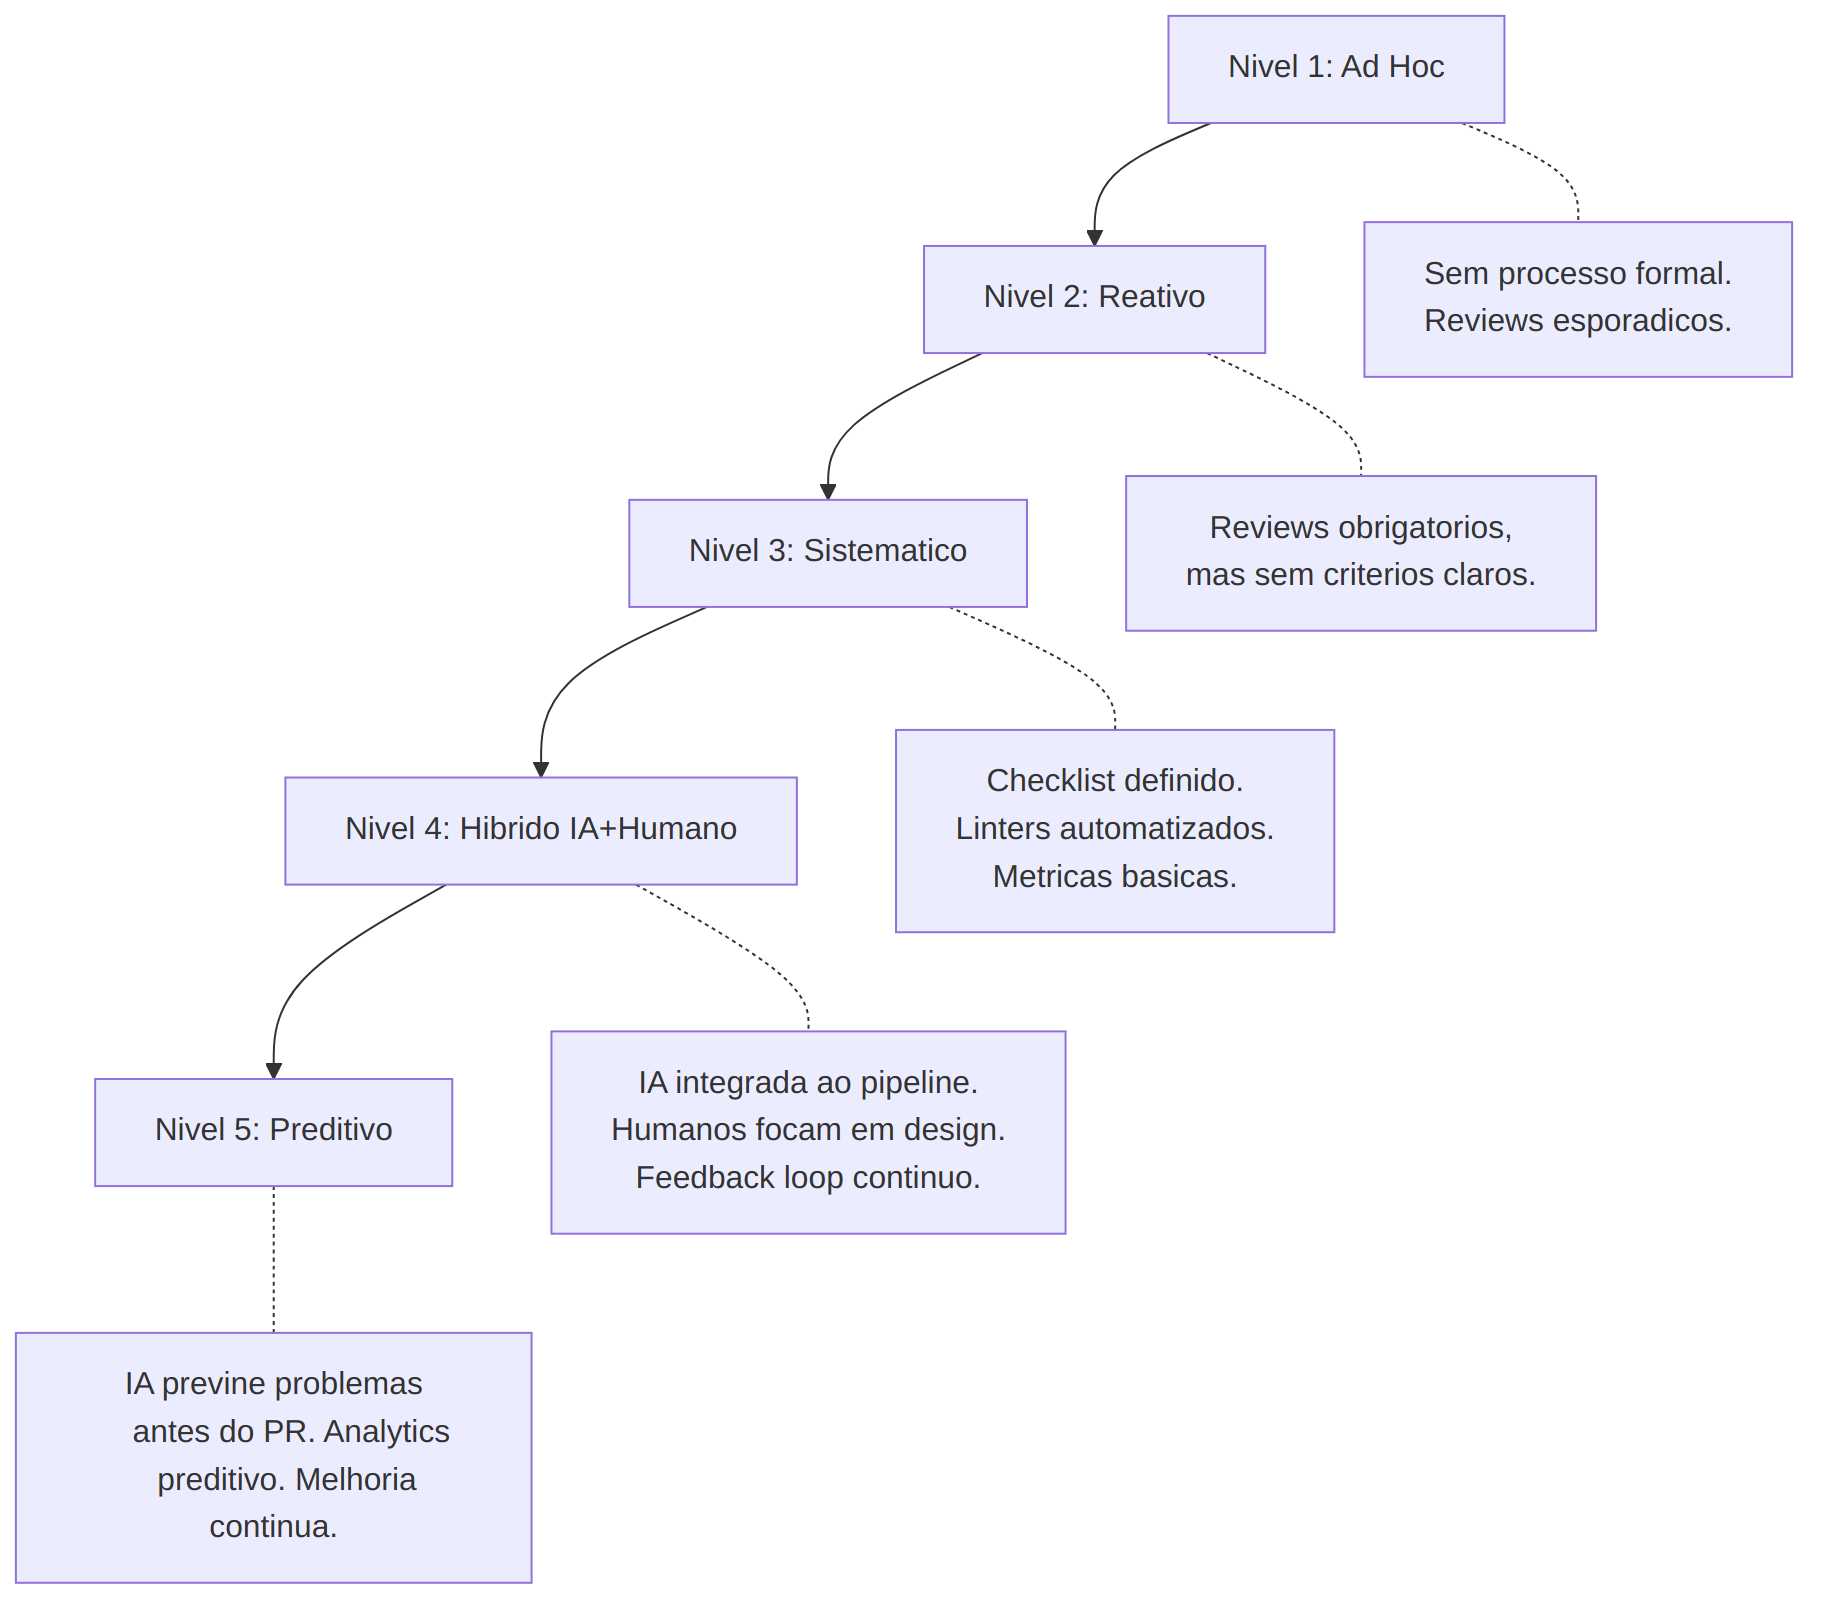
\includegraphics[width=0.85\textwidth]{imagens/06-revisao-codigo-era-ia-03-modelo-de-maturidade-em-code-review.png}
    \caption{Modelo de Maturidade em Code Review}
\end{figure}

% ============================================================
\section{Métricas e Melhoria Contínua}

O que não se mede, não se melhora. Mas cuidado: métricas mal escolhidas
incentivam comportamentos errados. Medir ``número de comentários por review''
incentiva comentários desnecessários. Medir ``tempo até aprovação'' incentiva
revisões superficiais.

\subsection{Métricas Recomendadas}

\begin{table}[htbp]
\centering
\caption{Métricas de Code Review}
\begin{tabular}{p{4cm}p{4cm}p{4cm}}
\toprule
\textbf{Métrica} & \textbf{O Que Mede} & \textbf{Meta Sugerida} \\
\midrule
Tempo médio até primeira revisão & Responsividade do time & $<$ 4 horas úteis \\
Tempo médio até merge & Eficiência do processo & $<$ 24 horas úteis \\
Tamanho médio do PR (linhas) & Disciplina de decomposição & 100--300 linhas \\
Taxa de bugs pós-merge & Eficácia da revisão & Tendência decrescente \\
Bugs encontrados em produção & Escapamento da revisão & $<$ 5\% dos deploys \\
Satisfação do time com reviews & Saúde cultural do processo & $>$ 7/10 \\
\% de PRs com revisão por IA & Adoção de automação & $>$ 90\% \\
Ciclos de revisão por PR & Clareza na comunicação & $<$ 3 ciclos \\
\bottomrule
\end{tabular}
\end{table}

\subsection{Bugs Encontrados Pós-Review em Produção}

\begin{itemize}
    \item Esta é a métrica mais importante: bugs que escaparam da revisão e
    chegaram a produção.
    \item Para cada bug em produção, faça um \textit{post-mortem} da revisão:
    o PR foi revisado? Por quantas pessoas? O que poderia ter sido detectado?
    \item Não use essa métrica para culpar revisores --- use para melhorar o
    processo.
    \item Categorize os escapamentos: era detectável por IA? Por humano? Por
    testes? Por nenhum (emergente)?
\end{itemize}

\subsection{Satisfação da Equipe}

\begin{itemize}
    \item Faça pesquisas trimestrais sobre a experiência de code review.
    \item Perguntas-chave:
    \begin{itemize}
        \item ``Você sente que os reviews são construtivos?''
        \item ``Você aprende com os reviews que recebe?''
        \item ``Os reviews são feitos em tempo razoável?''
        \item ``A IA está ajudando ou atrapalhando o processo?''
    \end{itemize}
    \item Se a satisfação está baixa, o processo precisa mudar ---
    independentemente de quão ``correto'' ele pareça.
\end{itemize}

\subsection{Throughput de Revisão}

\begin{itemize}
    \item Quantos PRs são revisados e mergeados por semana?
    \item Se o throughput cai, investigue: revisores sobrecarregados? PRs
    grandes demais? Falta de contexto nas descrições?
    \item O throughput ideal depende do tamanho do time, mas a tendência
    deve ser estável ou crescente.
\end{itemize}

\subsection{Melhoria Iterativa do Processo}

\begin{itemize}
    \item \textbf{Retrospectivas de review}: a cada sprint, discuta o que
    funcionou e o que não funcionou no processo de revisão.
    \item \textbf{Atualize o checklist}: conforme novos tipos de bugs
    escapam, adicione itens ao checklist.
    \item \textbf{Calibre a IA}: ajuste as regras e sensibilidade das
    ferramentas de revisão automática conforme o time evolui.
    \item \textbf{Rotacione revisores}: evite que sempre as mesmas pessoas
    revisem os mesmos módulos. Rotação distribui conhecimento.
    \item \textbf{Documente decisões}: quando uma discussão de review gera
    uma decisão importante, registre-a como ADR (Architecture Decision Record).
\end{itemize}

\begin{figure}[htbp]
    \centering
    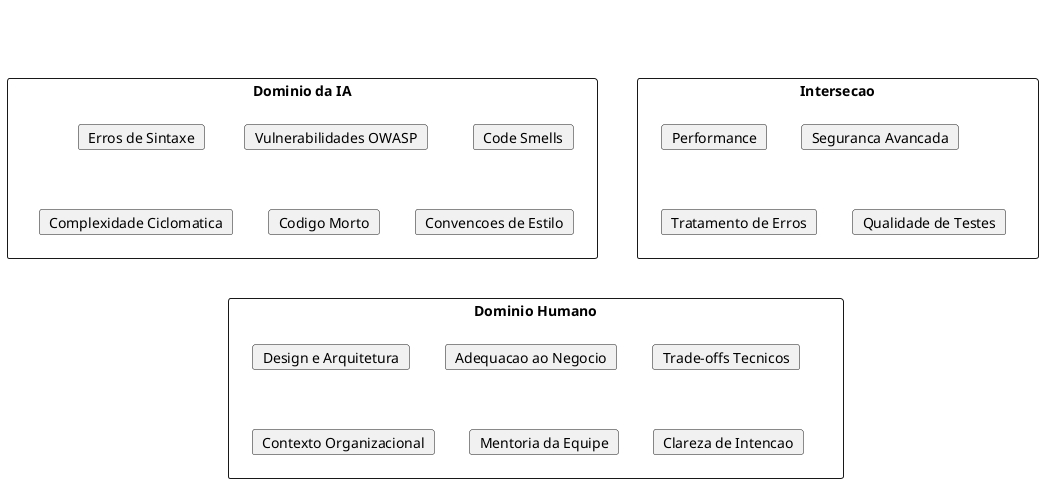
\includegraphics[width=0.85\textwidth]{imagens/06-revisao-codigo-era-ia-04-diagrama-o-que-ia-revisa-vs-o-que-humano-revisa.png}
    \caption{Diagrama: O Que IA Revisa vs O Que Humano Revisa}
\end{figure}

% ============================================================
\section{Conclusão}

Revisão de código na era da IA não é mais simples --- é mais sofisticada.
A IA elimina o trabalho tedioso de verificar sintaxe, convenções e padrões
conhecidos, liberando o revisor humano para o que realmente importa: avaliar
design, questionar decisões, entender contexto e ensinar.

\begin{itemize}
    \item \textbf{Revisão é sobre aprendizado coletivo}: o objetivo final não
    é apenas código melhor, mas um time melhor.
    \item \textbf{IA amplifica, não substitui}: ela é o melhor assistente que
    um revisor pode ter, mas a responsabilidade continua sendo humana.
    \item \textbf{Código gerado por IA exige mais rigor}: a armadilha do
    ``parece certo'' é real. Revisão de código de IA deve ser mais cuidadosa,
    não menos.
    \item \textbf{O processo evolui}: métricas, retrospectivas e feedback
    contínuo garantem que o processo de revisão acompanhe a evolução do
    time e das ferramentas.
    \item \textbf{Cultura importa mais que ferramentas}: a melhor ferramenta
    de revisão não salva um time com cultura tóxica de feedback. Invista
    em princípios antes de investir em automação.
\end{itemize}

Como disse Gerald Weinberg: ``Independentemente do que o problema pareça
ser, é sempre um problema de pessoas.'' Revisão de código não é diferente.

% ============================================================
\section*{Exercícios}

\begin{enumerate}
    \item \textbf{Revisão Comparativa}: submeta um mesmo Pull Request para
    revisão por uma ferramenta de IA (CodeRabbit, GitHub Copilot ou similar)
    e por um colega humano. Compare os feedbacks: o que cada um encontrou que
    o outro não encontrou? Documente as diferenças em categorias (segurança,
    design, performance, estilo).

    \item \textbf{Checklist Personalizado}: crie um checklist de revisão de
    código específico para o seu projeto atual. Inclua pelo menos 5 itens
    que são específicos do seu domínio de negócio (não genéricos). Use o
    checklist em 3 revisões reais e ajuste conforme necessário.

    \item \textbf{Caça ao Bug em Código de IA}: peça a uma IA para gerar
    a implementação de uma funcionalidade moderadamente complexa (ex.: sistema
    de autenticação com refresh tokens, ou processamento de pagamentos com
    retry). Revise o código gerado e documente pelo menos 3 problemas que a
    IA não identificaria sozinha. Classifique cada problema por severidade.

    \item \textbf{Descrição de PR}: escolha um PR recente do seu time que
    tinha uma descrição fraca ou inexistente. Reescreva a descrição seguindo
    o modelo apresentado neste capítulo (contexto, o que muda, decisões de
    design, como testar, checklist). Reflita: essa descrição teria tornado
    a revisão mais eficiente?

    \item \textbf{Análise de Métricas}: colete dados de code review do seu
    time nas últimas 4 semanas (tempo até primeira revisão, tamanho médio
    de PR, número de ciclos de revisão). Compare com as metas sugeridas
    neste capítulo. Identifique os 2 pontos de maior oportunidade de
    melhoria e proponha ações concretas.

    \item \textbf{Simulação de Revisão Híbrida}: configure uma pipeline de
    revisão automatizada em um repositório de teste usando GitHub Actions +
    uma ferramenta de revisão por IA. Submeta 3 PRs com defeitos intencionais
    (1 de segurança, 1 de performance, 1 de design). Verifique o que a
    automação detectou e o que escapou.
\end{enumerate}
